% ==============================================================================
% METADADOS DE VERSIONAMENTO E GOVERNANÇA DO PROJETO
% ==============================================================================
% Projeto: Revisão em Sistemas de Graduação em Escalada
% Arquivo: doc/revisao_graduacao/main.tex
% Status: Documento de Referência Técnica Pública (Acesso Aberto)
% Pipeline: Coleta inicial via Google Gemini Flash 3.8 (Deep Research) +
%           Refatoração, Auditoria de Fontes e Tipografia sob supervisão de Lu Freitas.
% ==============================================================================

\documentclass[11pt,a4paper]{article}
% Preâmbulo compartilhado dos documentos
\usepackage[utf8]{inputenc}
\usepackage[T1]{fontenc}
\usepackage[brazilian]{babel}
\usepackage{xcolor}
\usepackage{graphicx}
\usepackage{hyperref}
\newcommand{\docversion}{v3.0.0}
\newcommand{\docdate}{Novembro de 2026}

% Macros compartilhadas (highlights, siglas e metadados de IA)
% Será populado na Onda 2 com a macro de highlight pastel semitransparente.



\pagestyle{fancy}
\fancyhf{}
\fancyhead[L]{\small\color{secondary}Revisão em Sistemas de Graduação de Escalada}
\fancyhead[R]{\small\color{secondary}Normas, Aplicação e Fundamentos (\docversion)}
\fancyfoot[C]{\small\color{secondary}\thepage}
\renewcommand{\headrulewidth}{0.4pt}
\renewcommand{\footrulewidth}{0.4pt}

\title{\vspace{-1.6cm}\LARGE\textbf{\color{primary}Revisão em Sistemas de Graduação de Escalada}\\
\vspace{0.25cm}\Large\color{secondary}Normas, Aplicação e Fundamentos}

\author{\small\textbf{Supervisão Editorial e Design:} Lu Freitas\\
\footnotesize\color{secondary}Pesquisa, Estruturação e Auditoria Bibliográfica: Pipeline Multi-Agente de IA\\
\footnotesize\color{secondary}\textit{Documento de Referência Pública --- \docversion}}
\date{\small \docdate}

\begin{document}
\maketitle

\begin{abstract}
\noindent Este documento consolida uma revisão técnica, normativa e aplicada sobre sistemas de graduação de escalada em rocha e ginásios. Demonstra-se como federações internacionais (\textit{World Climbing}, UIAA, IRCRA), entidades nacionais (CBME e CBEscalada) e protocolos de \textit{route-setting} (Matriz RIC, ergonomia e \textit{forerunning}) reduzem a subjetividade dos graus. O texto principal organiza-se em três capítulos — (1) normas oficiais e redução da subjetividade, (2) aplicação prática em ginásios e (3) matrizes de equivalência e circuitos — seguidos de conclusão e três apêndices autocontidos (história das escalas, método científico IRCRA/RIC e glossário técnico).
\end{abstract}

\vspace{0.2cm}
\tableofcontents
\newpage

\section*{Introdução e Governança Metodológica}
\addcontentsline{toc}{section}{Introdução e Governança Metodológica}

A atribuição de graus na escalada cumpre três funções simultâneas:
\begin{enumerate}
    \item orientar a segurança do praticante diante do risco objetivo;
    \item fornecer uma métrica objetiva de progressão atlética;
    \item permitir comunicação padronizada entre diferentes regiões e ginásios.
\end{enumerate}
Sem compreensão da origem dessas escalas e dos métodos modernos de \textit{route-setting}, muros indoor tendem a reproduzir distorções de dificuldade e frustração pedagógica. Este documento público consolida o referencial técnico aplicável a ginásios e associações no Brasil, mantendo a numeração das seções alinhada diretamente aos três capítulos principais.

\subsection*{Uso Honesto de IA, Versionamento e Mitigação de Alucinações}
\begin{enumerate}
    \item \textbf{Papéis}: \textbf{Lu Freitas} atua na supervisão geral, design editorial e validação narrativa; sistemas de IA executam pesquisa documental, estruturação de tabelas e codificação \LaTeX{}.
    \item \textbf{Pipeline e Versionamento}: O levantamento inicial de fontes foi realizado pelo \textbf{Google Gemini Flash 3.8} (\textit{Deep Research}). A partir da v2.0, agentes independentes auditam documentos primários e operam sob controle de versão semântico (\texttt{\docversion}) com registro rastreável no código-fonte.
    \item \textbf{Rastreabilidade}: O texto distingue explicitamente \textbf{Norma Literal/Citação Direta} (com página e seção), \textbf{Paráfrase Técnica} e \textbf{Interpretação Analítica}, omitindo qualquer dado não verificável nas fontes lidas.
\end{enumerate}

\clearpage
% EDITORIAL QUESTION: Como as federações internacionais e nacionais dividem competências normativas e quais ferramentas científicas reduzem a subjetividade do route-setting?
\section{Normas Oficiais, Governança e Redução da Subjetividade}

A organização da escalada divide-se entre entidades voltadas ao montanhismo em rocha natural e federações dedicadas ao esporte de competição em estruturas artificiais.

\subsection*{1.1 Hierarquia Internacional: UIAA, World Climbing (ex-IFSC), COI e CPI}

% SOURCE [VERIFIED_PRIMARY]: UIAA History (https://www.theuiaa.org/inside-the-uiaa/history/); World Climbing About & Rebrand 10/12/2025 (https://www.worldclimbing.com/ifsc, https://www.worldclimbing.com/news/world-climbing-launches-new-global-identity).
\begin{itemize}
    \item \textbf{UIAA}: Fundada em agosto de 1932 em Chamonix, atua na certificação de segurança de equipamentos (\textit{UIAA Safety Label}), ética de acesso em montanha, preservação ambiental e competições de escalada no gelo \cite{uiaa_history}. Administrou as Copas do Mundo de escalada esportiva de 1989 a 2006 \cite{worldclimbing_about}.
    \item \textbf{World Climbing (antiga IFSC)}: Fundada em 27 de janeiro de 2007 em Frankfurt como \textit{International Federation of Sport Climbing} (IFSC) para viabilizar a autonomia olímpica da modalidade. Em \textbf{10 de dezembro de 2025}, adotou oficialmente o nome \textbf{World Climbing} e rebatizou o circuito mundial para \textit{World Climbing Series} a partir de 2026 \cite{worldclimbing_about, worldclimbing_rebrand}.
    \item \textbf{COI e CPI}: Reconhecida pelo Comitê Olímpico Internacional (COI) desde 2010 e pelo Comitê Paralímpico Internacional (CPI). Estreou em Tóquio 2020 (formato combinado), dividiu-se em duas disputas em Paris 2024 e terá medalhas independentes para as três disciplinas em Los Angeles 2028, além da estreia paralímpica da \textbf{Paraescalada} \cite{worldclimbing_about}.
\end{itemize}

\subsection*{1.2 As Quatro Disciplinas da World Climbing e o Setting de Competição}

% SOURCE [VERIFIED_PRIMARY]: World Climbing / IFSC Rules 2025 (https://www.worldclimbing.com/commissions/routesetters) & Paraclimbing Classification Rules.
A World Climbing regulamenta quatro categorias oficiais \cite{worldclimbing_about, ifsc_rules}:
\begin{enumerate}
    \item \textbf{Boulder}: Blocos curtos em paredes de até 4,5\,m, sem corda, sobre tatames contínuos, pontuando por \textit{Tops}, \textit{Zones} e número de tentativas em janelas de tempo fixas.
    \item \textbf{Guiada (\textit{Lead})}: Vias de no mínimo 15\,m em tentativa única (\textit{onsight}) com limite de 6 minutos, costurando proteções fixas.
    \item \textbf{Velocidade (\textit{Speed})}: Duelo simultâneo em parede padronizada de 15\,m a $5^\circ$ negativos com agarras e posições idênticas globalmente.
    \item \textbf{Paraescalada (\textit{Para Climbing})}: Disputas em \textit{top-rope} divididas por classes funcionais (B1--B3, AU/AL, RP1--RP3) \cite{ifsc_paraclimbing}.
\end{enumerate}

Diferentemente dos ginásios comerciais, \textbf{competições oficiais da World Climbing não atribuem grau numérico público às vias} \cite{ifsc_rules}. A Comissão de \textit{Setters} designa um \textit{Head Setter} certificado cujo objetivo é produzir \textbf{separação estatística} no pódio, equilibrando estilos distintos (coordenação dinâmica, força em negativo, equilíbrio em placa e complexidade mista) com largada obrigatória em quatro fitas \cite{ifsc_rules}.

\subsection*{1.3 Cenário Institucional no Brasil: CBEscalada vs. CBME}

% SOURCE [VERIFIED_PRIMARY]: CBEscalada Sobre & Filiações 2026 (https://cbescalada.org.br/entidade/9/sobre, https://cbescalada.org.br/atletas/74/filiacoes); CBME DT-2016/01 p. 1.
\begin{itemize}
    \item \textbf{CBEscalada}: Fundada em 2014 (originalmente ABEE), é a associação civil que detém a gestão exclusiva da escalada esportiva de competição no Brasil, integrando o Sistema Nacional do Desporto (Lei nº 14.597/2023) \cite{cbescalada_sobre}. Filiada à World Climbing e reconhecida pelo COB e CPB, opera o Centro de Treinamento Nacional em Curitiba e homologa pódios nacionais junto ao Ministério do Esporte para o programa \textbf{Bolsa Atleta} e editais de fomento como o \textit{Projeto Técnicos de Base} \cite{cbescalada_sobre, cbescalada_filiacoes}.
    \item \textbf{CBME}: Entidade máxima do montanhismo e escalada em rocha no Brasil, filiada à UIAA, que congrega federações estaduais e associações regionais (como FEMERJ, FEMESP, FGM, FEPAM, FEMEMG, FEMECE, ACE, AEP, APE e AERN) \cite{cbme_dt01}. Regula diretrizes técnicas de graduação em rocha (DT-2016/01), ética de conquista (DT-2016/10) e manejo ambiental \cite{cbme_dt01, cbme_dt10}.
\end{itemize}

\subsection*{1.4 A Norma CBME DT-2016/01 e o Grau ``À Vista'' vs. ``Grau Trabalhado''}

% SOURCE [VERIFIED_PRIMARY]: CBME DT-2016/01 (03/12/2016), págs. 1, 2 e 5 (https://cbme.org.br/novo/wp-content/uploads/2025/03/CBME-DT-2016_01-Sistema-Brasileiro-de-graduacao-de-vias-de-escalada.pdf).
A \textbf{Diretriz Técnica CBME DT-2016/01} estabelece o sistema brasileiro de graduação em rocha \cite{cbme_dt01}. O quadro abaixo reproduz três trechos determinantes do documento original:

\facsimilebox{EXCERTO DOCUMENTAL VERIFICADO --- CBME: DT-2016/01 (03/12/2016, Páginas 1, 2 e 5)}{%
\textbf{[Página 1 --- Cabeçalho e Entidades Filiadas]}: ``CONFEDERAÇÃO BRASILEIRA DE MONTANHISMO E ESCALADA --- CBME. Documento: CBME: DT-2016/01. Data criação: 03 de dezembro de 2016. Nota: Substitui o sistema de graduação aprovado por Assembleia Geral em 25/08/2007. Entidades filiadas: FGM, FEPAM, FEMESP, FEMERJ, FEMEMG, FEMECE e as Associações ACE, AEP, APE e Associação de Escaladores do Rio Grande do Norte (AERN).''\\[4pt]
\textbf{[Página 2 --- Seção 2. INTRODUÇÃO]}: ``Uma das vantagens do sistema brasileiro é a menção dos graus geral e do lance mais difícil da via em separado (...). \textbf{Lembramos que na atribuição do grau a uma via considera-se que o escalador está guiando e escalando `à vista', isto é, sem conhecimento prévio da via.}''\\[4pt]
\textbf{[Página 5 --- Seção 3.3. Vias de Uma Enfiada, Falésias e Boulders]}: ``Para estas vias não há sentido em se atribuir um grau geral e um grau para o lance mais difícil, uma vez que são vias curtas, de comprimento máximo de 50 ou 60 metros. \textbf{Então o grau geral é abolido, e utiliza-se somente o grau do lance ou sequência mais difícil, em romanos, para expressar a sua dificuldade.} (...) Esta graduação é válida para boulders, falésias e vias curtas em geral.''
}

\subsubsection*{Grau Geral, Crux e o Efeito do Grau Trabalhado (``Decotar'' a Via)}

% SOURCE [INTERPRETATION]: Análise cultural derivada de CBME DT-2016/01 (págs. 2--5, 13) e convenções de boulder em Hueco/Fontainebleau.
\begin{enumerate}
    \item \textbf{Parede Tradicional vs. Boulder}: Em vias longas (\textit{multi-pitch}), o \textbf{Grau Geral} (arábicos ordinais) expressa o comprometimento contínuo e o \textbf{Grau do Crux} (romanos com \textit{sup} até VIsup e letras \textit{a, b, c} a partir de VIIa) indica o passo mais difícil \cite{cbme_dt01}. Em falésias curtas e boulders, a Seção 3.3 (pág. 5) abole o Grau Geral, adotando apenas o crux (ou a Escala $V$ na prática de campo brasileira) \cite{cbme_dt01, guia_cocalzinho, guia_igatu}.
    \item \textbf{À Vista (\textit{Onsight}) vs. Grau Trabalhado (``Decotado'')}: A CBME fixa o grau sob a premissa da escalada \hlkey{``à vista'' (\textit{onsight})} \cite{cbme_dt01}. Quando o escalador ensaia a sequência repetidamente, memoriza micro-apoios e automatiza o gesto motor até encadeá-la sem hesitação, pratica o \hlwork{\textbf{grau trabalhado} (ou ``decotar'' a via, do francês \textit{décoter})}.
    \item \textbf{Choque Cultural em Ginásios}: Enquanto a parede tradicional cobra o erro de leitura sob exposição, o boulder moderno internacional gradua assumindo o \hlwork{\textbf{grau trabalhado / projeto (\textit{redpoint})}}. Em ginásios, um bloco baseado apenas em um truque de leitura (\textit{beta} oculto) parece dois graus mais duro na primeira tentativa e despenca de dificuldade após ser decotado — exigindo que os \textit{setters} não superestimem graus baseados em enigmas visuais.
\end{enumerate}

\subsection*{1.5 Ferramentas Científicas para Setters: Escala IRCRA}

% SOURCE [VERIFIED_PRIMARY]: Draper et al. (2016), Sports Technology 8(3-4), págs. 85--93 (https://ircra.rocks/reporting-grades-in-climbing-research/).
Existem instrumentos científicos criados para medir e comparar graduações de escalada sem depender da percepção isolada de um único avaliador. A \textbf{IRCRA} desenvolveu uma escala numérica inteira universal (1 a 32, posteriormente expandida até 39 na literatura) para viabilizar análises estatísticas entre sistemas incompatíveis como YDS, Font e $V$-Scale \cite{ircra_draper, pmc_ric_study}.

Para \textit{setters} e gestores de ginásios, embora a IRCRA nunca vá impressa nas etiquetas da parede, ela oferece um diagnóstico prático decisivo: \textbf{revela a não linearidade oculta da Escala $V$} \cite{ircra_draper, youthclimbing_conv}. Entre VB (IRCRA 9) e V1 (IRCRA 14) existem cinco degraus inteiros de exigência motora, enquanto de V1 a V3 avança-se apenas um degrau IRCRA por nível (detalhamento formal e limites científicos no Apêndice~B).

\subsection*{1.6 Redução da Subjetividade: Matriz RIC, Ergonomia e Forerunning}

% SOURCE [VERIFIED_PRIMARY]: PMC11881084 (2024), págs. 2--5 (https://pmc.ncbi.nlm.nih.gov/articles/PMC11881084/); Anderson (2014), caps. 3 e 5; CWA (2023).
Para reduzir a dependência do biotipo, protocolos técnicos de \textit{route-setting} utilizam três barreiras de controle \cite{cwa_setting, anderson_routesetting, pmc_ric_study}:
\begin{enumerate}
    \item \textbf{Matriz RIC (Risco, Intensidade e Complexidade)}: Proposta por Godoffe e Katiyo e formalizada em estudos recentes \cite{godoffe_routesetting, pmc_ric_study}, atribui notas de 1 a 5 a três eixos independentes: \textbf{Risco ($R$)} (comprometimento espacial/queda), \textbf{Intensidade ($I$)} (carga física/força de dedos) e \textbf{Complexidade ($C$)} (leitura e coordenação). Isso garante que estilos opostos (placa técnica vs. teto de força) convirjam para o mesmo grau nominal \cite{agility_ric}.
    \item \textbf{Ergonomia e Controle Morfológico}: Conforme Anderson \cite{anderson_routesetting}, evita-se fabricar dificuldade por meio de posições lesivas (como arqueamento fechado em graus iniciais) e neutraliza-se o viés de envergadura com apoios intermediários de pé ou agarras duplas \cite{paraclimbing_guide}.
    \item \textbf{Forerunning Coletivo e Consenso}: A CWA estabelece que nenhum bloco seja graduado por um único \textit{setter} \cite{cwa_setting}. A testagem prévia por múltiplos escaladores de estaturas distintas corrige quebras de sequência (\textit{beta breaks}), complementada por auditoria estatística via aplicativos digitais após repetições do público \cite{rockrealms_home, topclimbing_platform}.
\end{enumerate}

\noindent\textit{Síntese:} A normatização institucional (World Climbing, CBME, CBEscalada) delimita o escopo de cada escala, enquanto a combinação de IRCRA (diagnóstico linear), Matriz RIC (equilíbrio de estilos) e \textit{forerunning} coletivo transforma a graduação de opinião individual em processo auditável.


\clearpage
% EDITORIAL QUESTION: Como os ginásios contemporâneos traduzem escalas de rocha para circuitos físicos, evitam gargalos na base e calibram sua dificuldade?
\section{Aplicação Prática da Graduação em Ginásios Contemporâneos}

Ao transpor escalas de rocha para muros indoor, ginásios precisam conciliar três demandas: otimizar o estoque financeiro de agarras, acolher iniciantes sem risco de lesão e manter fidelidade com a rocha para praticantes avançados.

\subsection*{2.1 Arquitetura Física de Sinalização}

% SOURCE [VERIFIED_PRIMARY]: CBJ (2019/2023) (https://climbingbusinessjournal.com/tape-to-no-tape-in-6-steps/); CWA Colors (2022).
Levantamentos da CWA e do CBJ classificam três modelos físicos de sinalização \cite{cbj_tape, cwa_colors}:
\begin{enumerate}
    \item \textbf{Monocromático por Cor de Agarra (\textit{Hold Color})}: Todas as agarras do bloco têm a mesma cor de resina. Oferece leitura visual limpa, porém exige alto investimento de capital para replicar formatos em todas as cores \cite{cbj_tape}.
    \item \textbf{Fitas Adesivas (\textit{Taped Circuits})}: Agarras de qualquer cor são instaladas livremente e demarcadas por fita colorida na parede. Exige manutenção periódica das fitas, mas confere ao \textit{setter} liberdade total para usar o melhor formato biomecânico do estoque \cite{cwa_colors}.
    \item \textbf{Etiquetas de Base (\textit{Start Tags})}: Placa na largada indicando número do bloco, cor do circuito, subgrau, \textit{setters} e data de montagem \cite{bmc_grades, reddit_hangar}.
\end{enumerate}

\subsection*{2.2 Faixas Sobrepostas e o Dilema da Base}

% SOURCE [VERIFIED_PRIMARY]: Bouldering Project (2023); CWA (2023); Draper et al. (2016).
A maioria dos ginásios adota \textbf{faixas sobrepostas de graduação} (\textit{overlapping bands}, como Verde = V2/V3 e Azul = V3/V4) para absorver variações de estilo entre placa, vertical e teto \cite{bp_grades, womens_gradient}.

\boxhighlight{Lógica das Faixas Sobrepostas}{Uma faixa de dois graus cria transição suave entre circuitos: quem domina o topo da faixa anterior já executa os blocos de entrada da cor seguinte, reduzindo bloqueios psicológicos \cite{bp_grades}.}

Entretanto, a combinação das diretrizes da CWA com a escala IRCRA impõe uma \textbf{regra crítica de exceção para o circuito inicial} \cite{cwa_setting, ircra_draper}:
\begin{itemize}
    \item A partir de V2/V3 a sobreposição de dois graus funciona com precisão; \textbf{entre VB, V0 e V1, porém, agrupar tudo em uma única faixa gera distorção pedagógica severa}.
    \item Como VB (IRCRA 9) a V1 (IRCRA 14) abrange cinco níveis inteiros de aptidão motora, um iniciante no primeiro dia sobe um VB em jarros, mas não possui adaptação tendínea para um V1 real de rocha (equivalente a Font 6A / CBME VIIa) \cite{ircra_draper, cbme_dt01}.
    \item Recomenda-se isolar o nível introdutório (VB/V0-) em faixa própria ou adotar \textbf{sub-identificadores na etiqueta de base} para separar blocos de iniciação pura dos blocos de transição \cite{cwa_setting, topclimbing_platform}.
\end{itemize}

\subsection*{2.3 Benchmarking Internacional e Análise de Quadros de Referência}

% SOURCE [VERIFIED_PRIMARY]: Bouldering Project, Arkose, CityROCK (2020), TopClimbing; quadros visuais coletados de Peak Experiences, The Front, Aliior, Sportrock, Rockfish e J2 Bouldering.
A Tabela~\ref{tab:benchmarking_gyms} resume o modelo operacional de redes internacionais e brasileiras, e a Figura~\ref{fig:quadros_referencia} ilustra seis exemplos reais de quadros murais analisados na revisão.

\begin{table}[!htbp]
\centering
\caption{Benchmarking de sistemas de graduação em ginásios internacionais e brasileiros.}
\label{tab:benchmarking_gyms}
\footnotesize
\renewcommand{\arraystretch}{1.12}
\begin{tabularx}{\linewidth}{p{2.6cm}p{2.1cm}p{2.8cm}X}
\toprule
\textbf{Ginásio / Rede} & \textbf{Localização} & \textbf{Sinalização} & \textbf{Estrutura de Faixas e Governança} \\
\midrule
\textbf{Bouldering Project} & EUA & Monocromático & 9 circuitos com sobreposição de 3 graus $V$ (Amarelo VB--V1 até Branco V7--V9) \cite{bp_grades, gearloop_tempe}. \\
\rowcolor{rowgray}
\textbf{Arkose} & França & Monocromático (Font) & 6 cores sem sobreposição nominal direta (Amarelo Font 4 até Roxo 7C+) \cite{arkose_niveaux}. \\
\textbf{The Climbing Hangar} & Reino Unido & Monocromático + Tags & 7 circuitos progressivos (Cinza/Verde VB--V0 até Preto V7+); auditoria via app Griptonite \cite{bmc_grades, reddit_hangar}. \\
\rowcolor{rowgray}
\textbf{CityROCK} & África do Sul & Híbrido (Presas + Tags) & Pareamento entre circuitos cromáticos, Escala $V$ (calibrada com Rocklands) e Ewbank para corda \cite{cityrock_guide}. \\
\textbf{90 Graus / Casa de Pedra} & Brasil & Fitas, Tags ou Monocromático & Faixas de 1 a 2 graus $V$, calibradas com rocha nacional (Cocalzinho/Igatu) e integradas ao app TopClimbing \cite{topclimbing_platform, aventura_retrato}. \\
\bottomrule
\end{tabularx}
\end{table}

\begin{figure}[!htbp]
\centering
\caption{Exemplos visuais de quadros de graduação em ginásios internacionais (referências para análise crítica de legibilidade, sobreposição e faixa de entrada).}
\label{fig:quadros_referencia}
\footnotesize
\begin{tabular}{ccc}
\IfFileExists{../../references/charts/chart_01_peak_experiences.jpg}{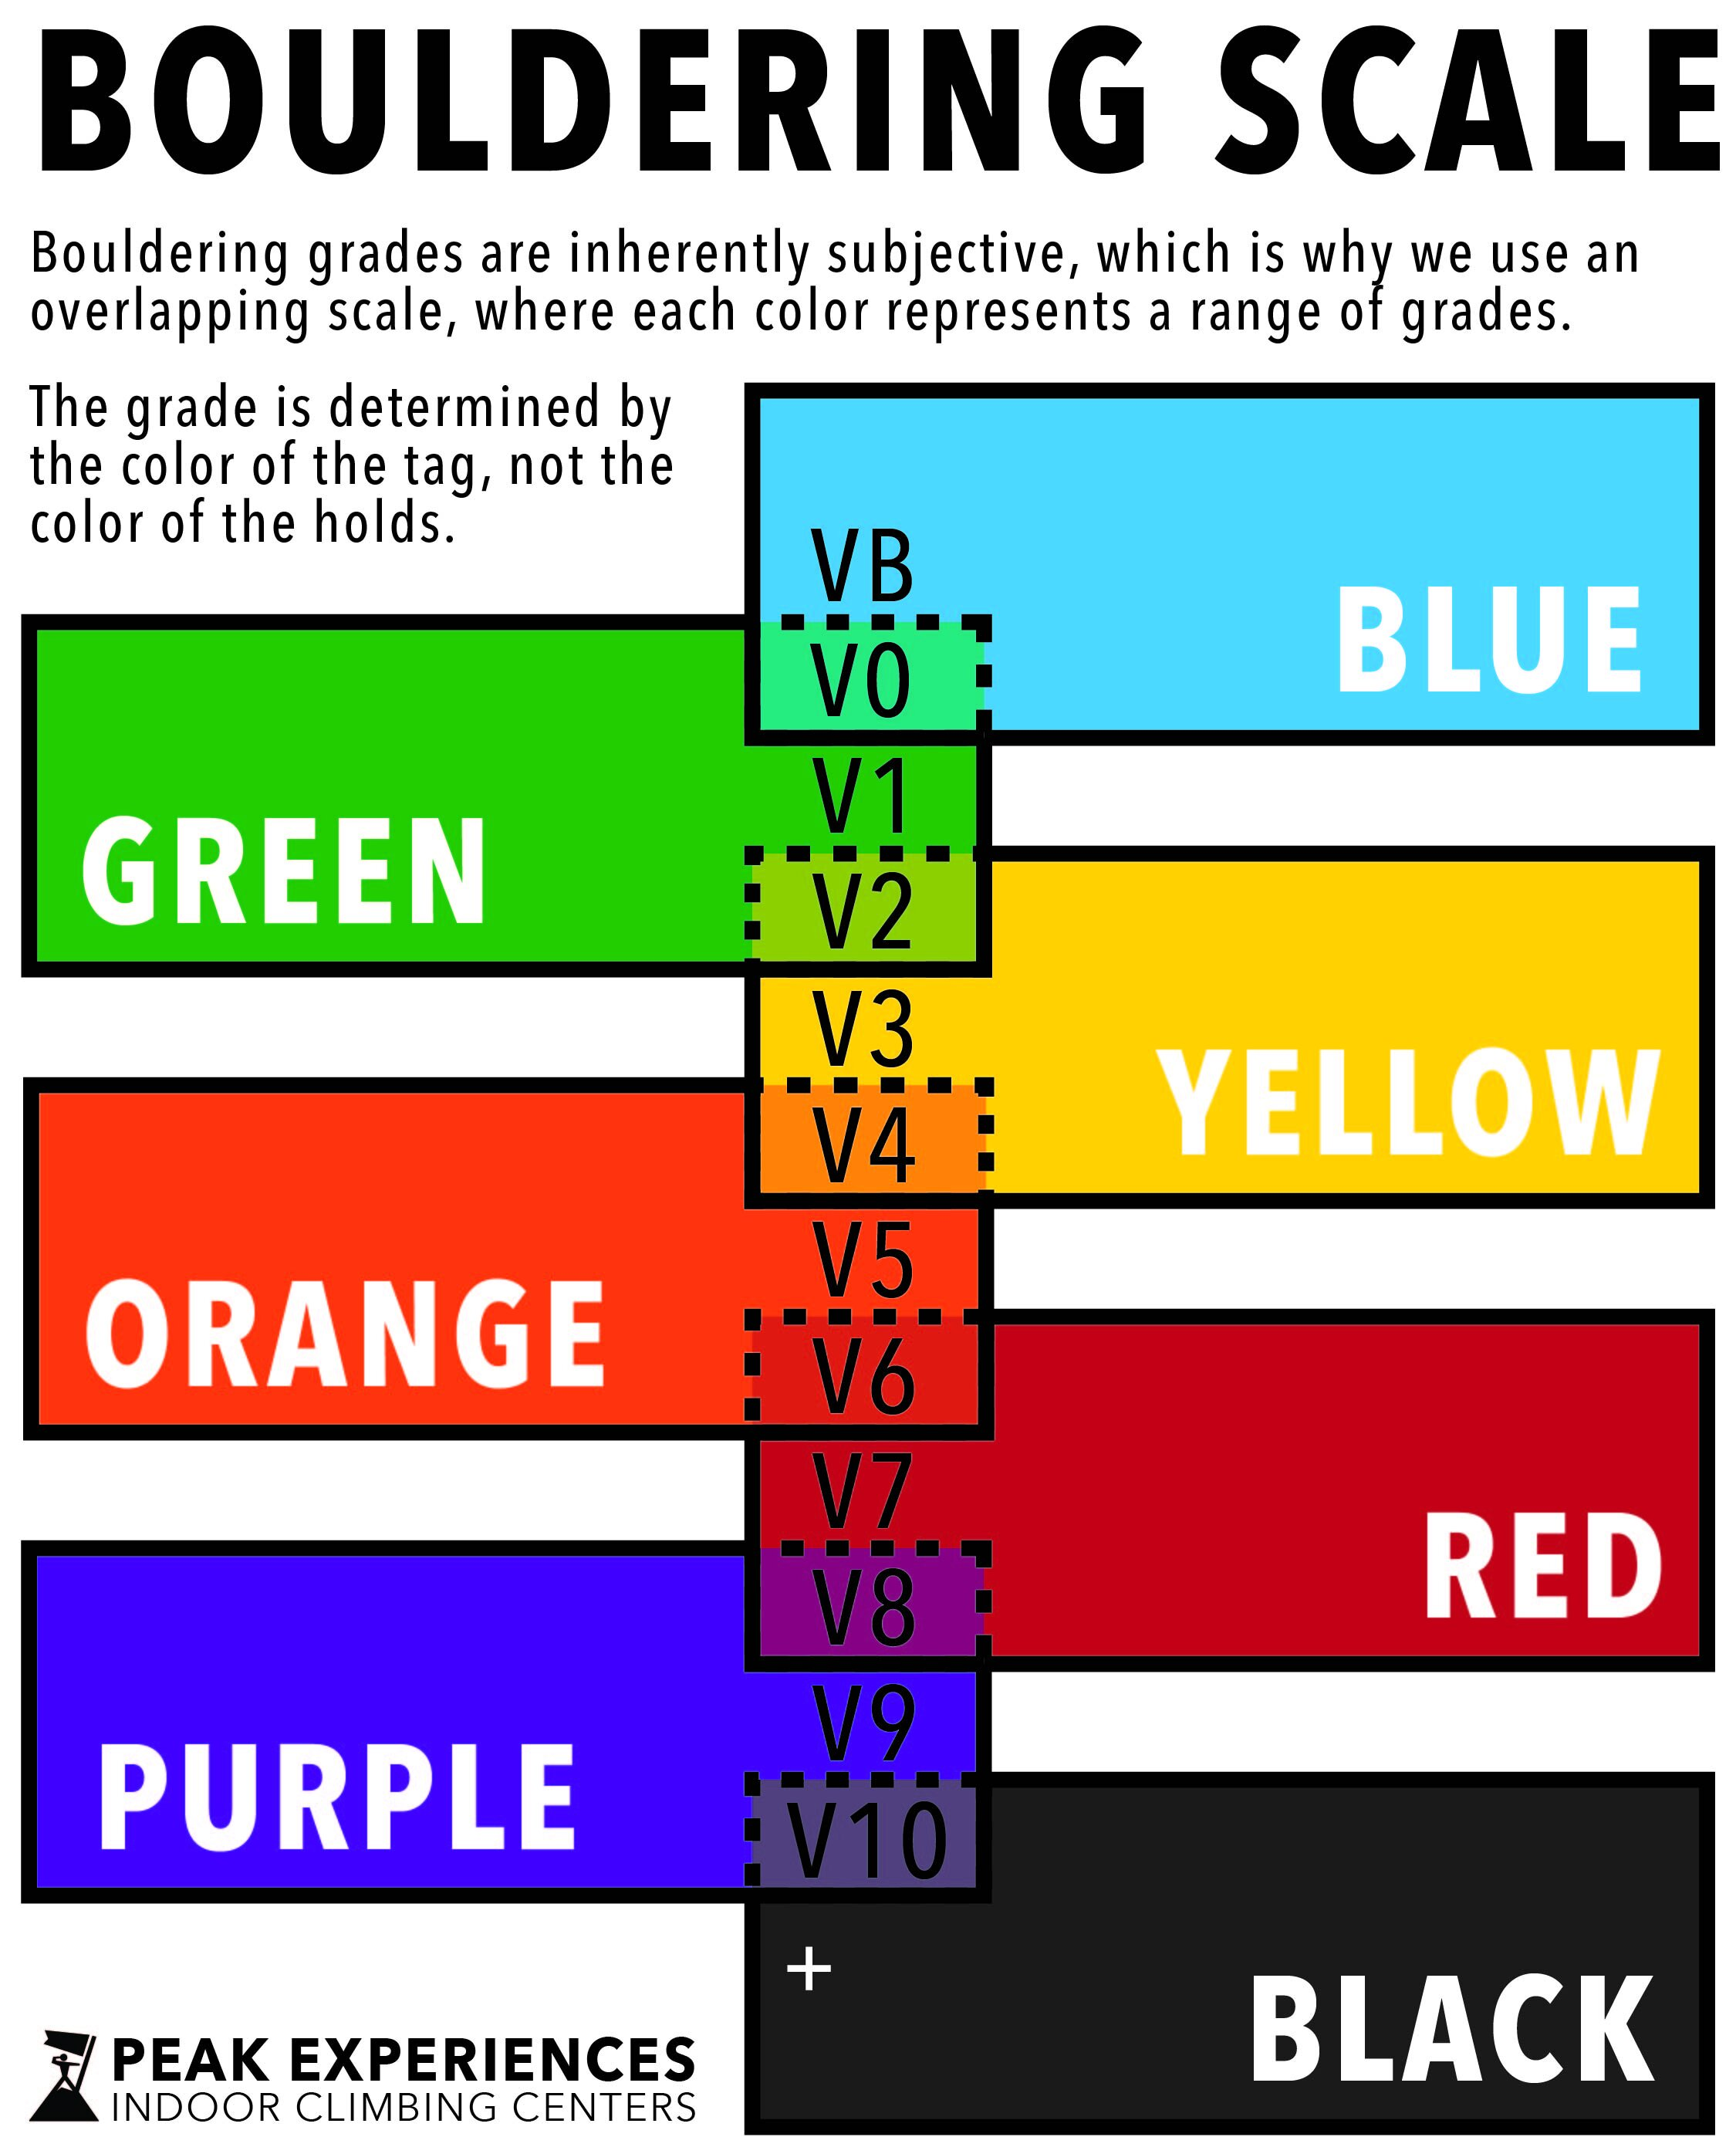
\includegraphics[width=0.30\linewidth]{../../references/charts/chart_01_peak_experiences.jpg}}{\fbox{\parbox[c][3cm]{0.28\linewidth}{\centering Peak Experiences\\(\texttt{chart\_01\_peak\_experiences.jpg})}}} &
\IfFileExists{../../references/charts/chart_02_the_front.jpg}{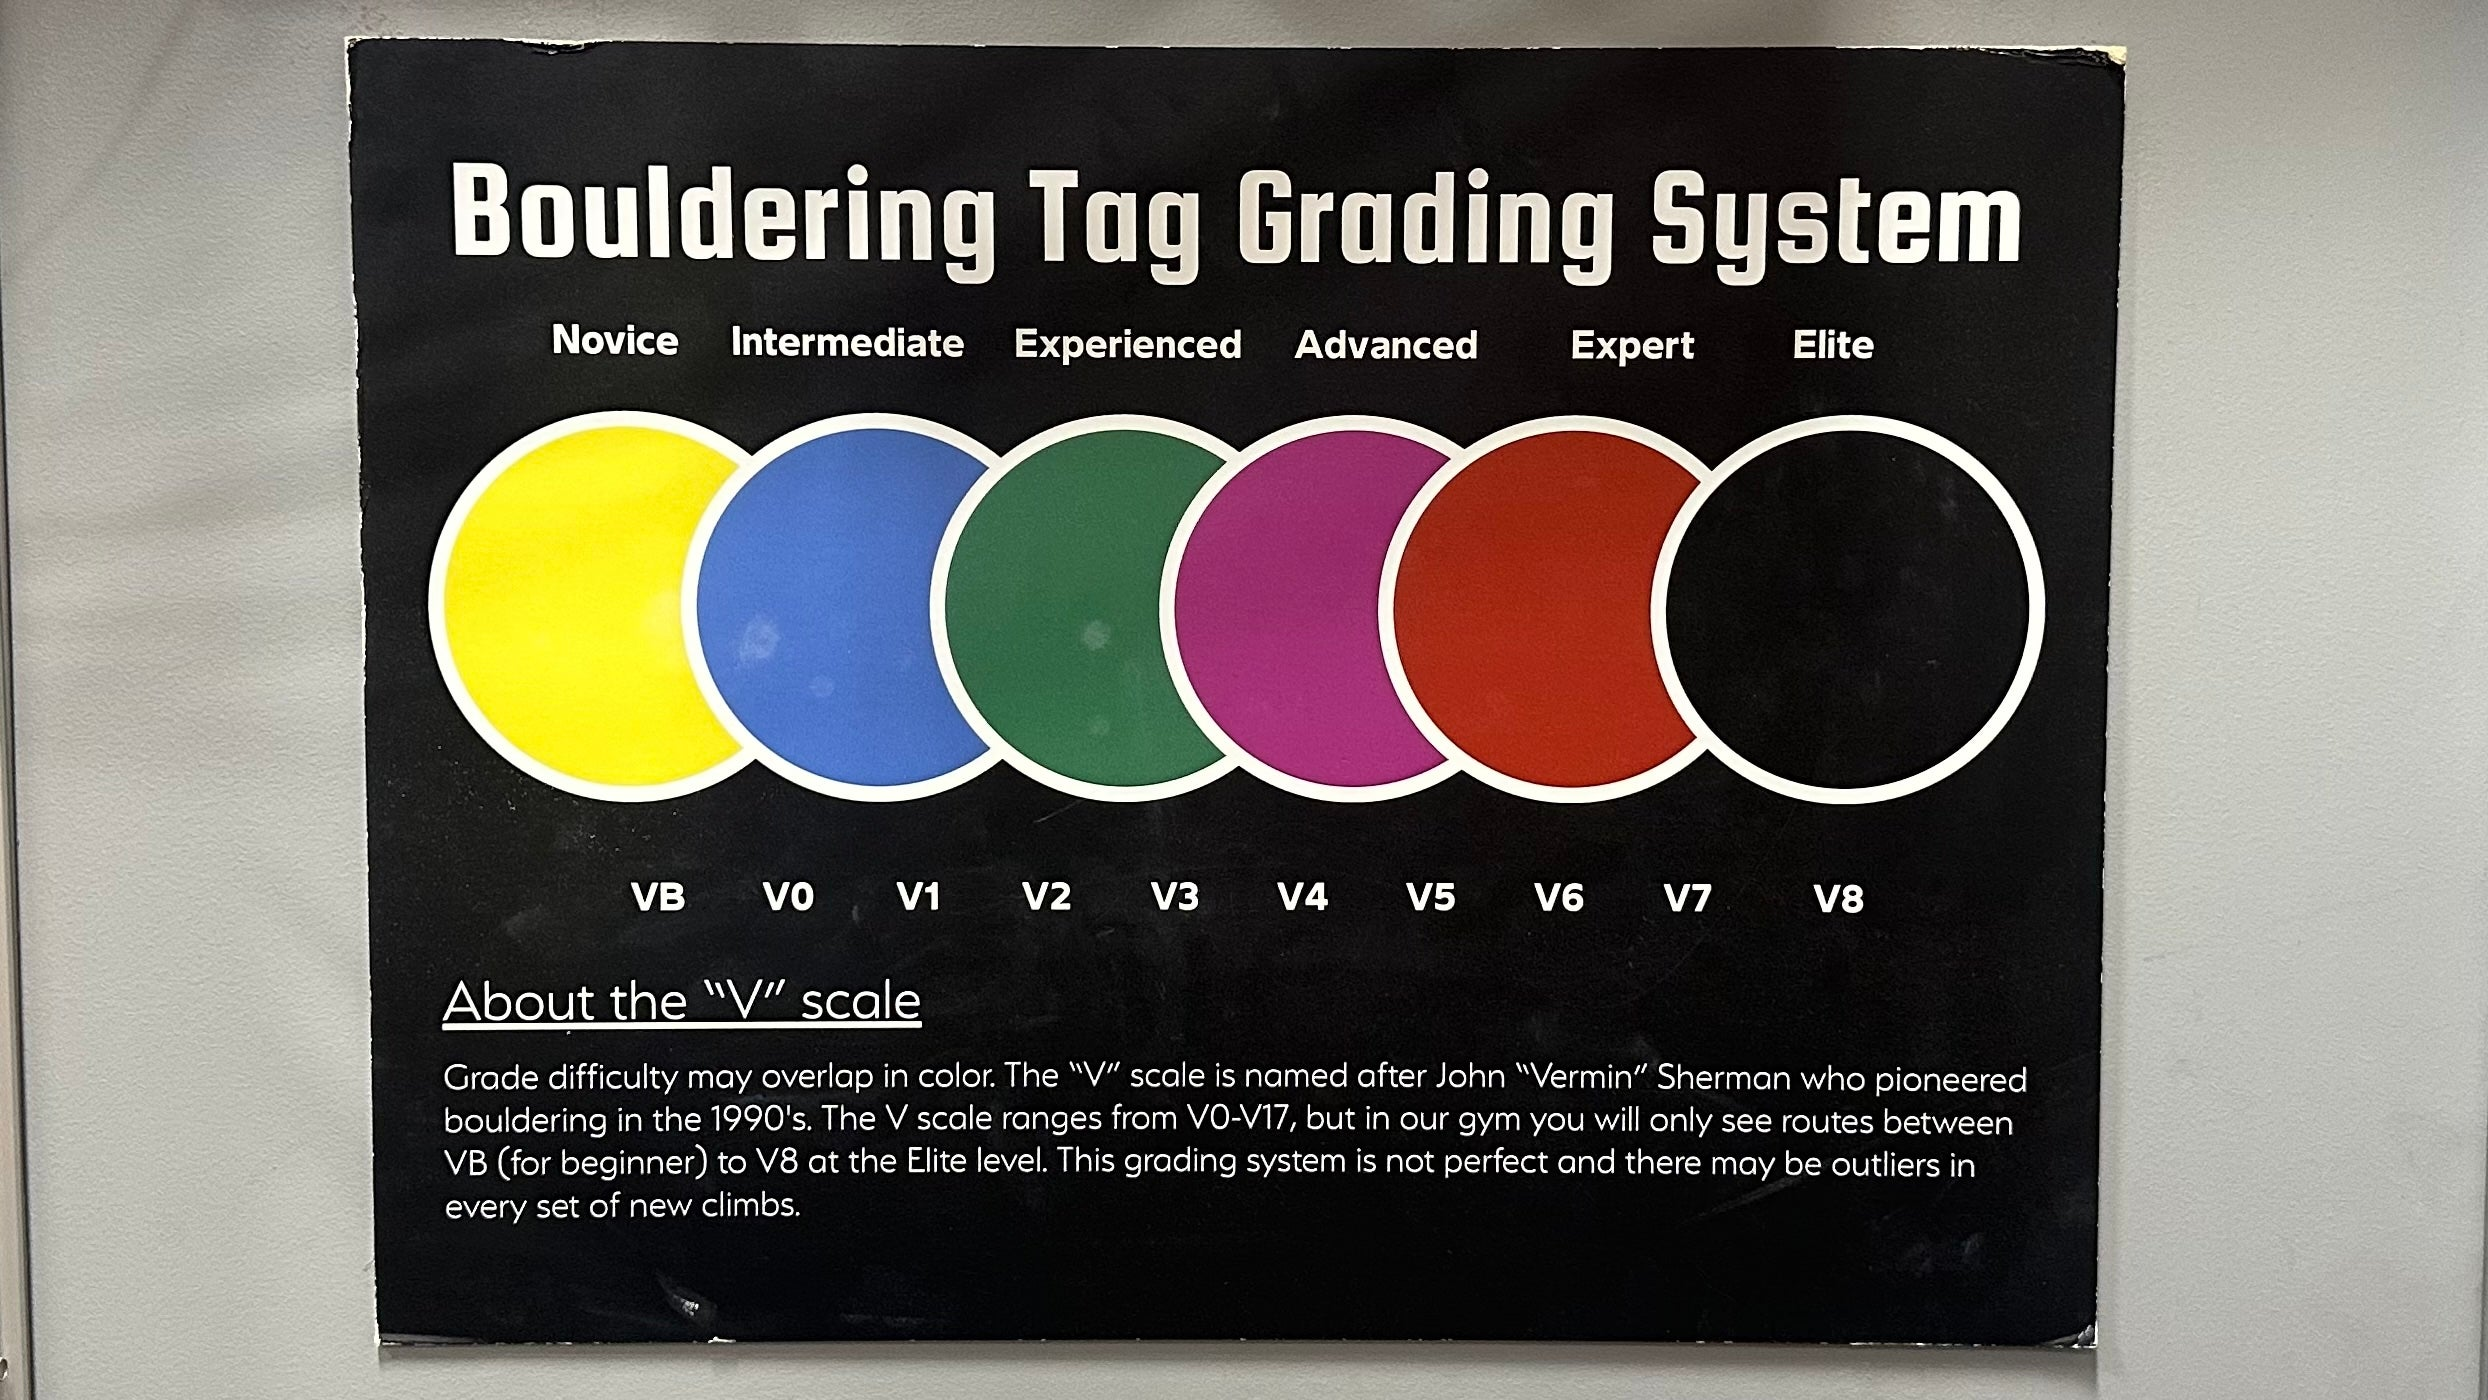
\includegraphics[width=0.30\linewidth]{../../references/charts/chart_02_the_front.jpg}}{\fbox{\parbox[c][3cm]{0.28\linewidth}{\centering The Front (Dot System)\\(\texttt{chart\_02\_the\_front.jpg})}}} &
\IfFileExists{../../references/charts/chart_03_aliior_jp.jpg}{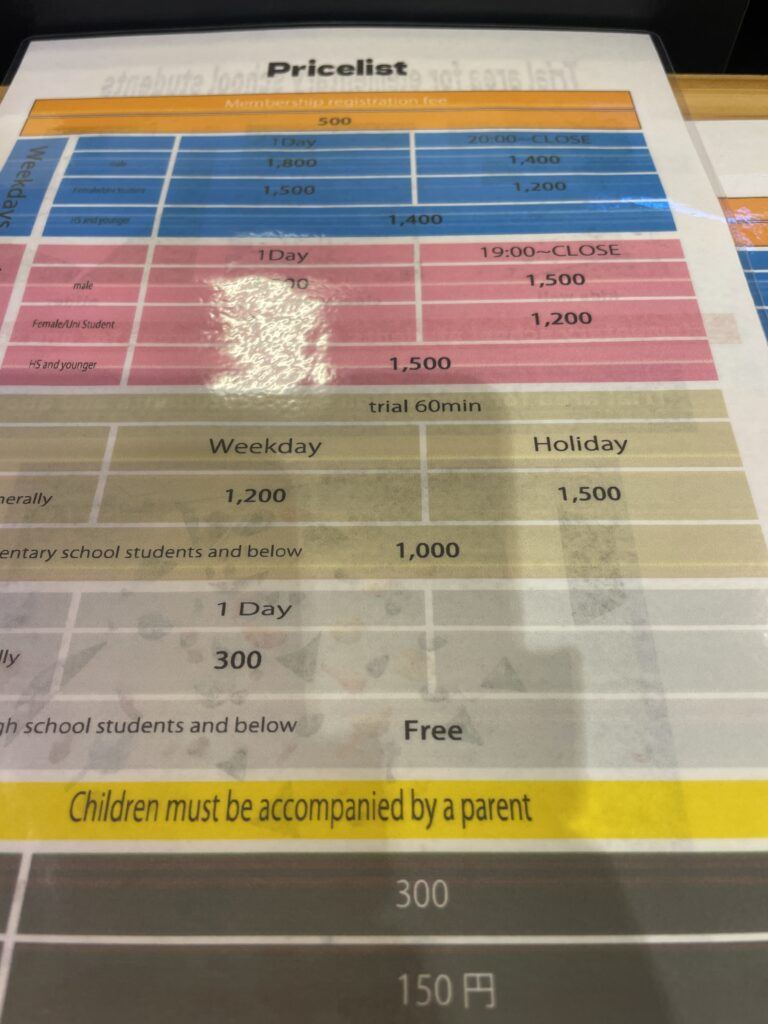
\includegraphics[width=0.30\linewidth]{../../references/charts/chart_03_aliior_jp.jpg}}{\fbox{\parbox[c][3cm]{0.28\linewidth}{\centering Aliior Japão (Kyu/Dan)\\(\texttt{chart\_03\_aliior\_jp.jpg})}}} \\[4pt]
(a) Peak Experiences & (b) The Front & (c) Aliior (Japão) \\[8pt]
\IfFileExists{../../references/charts/chart_04_sportrock.png}{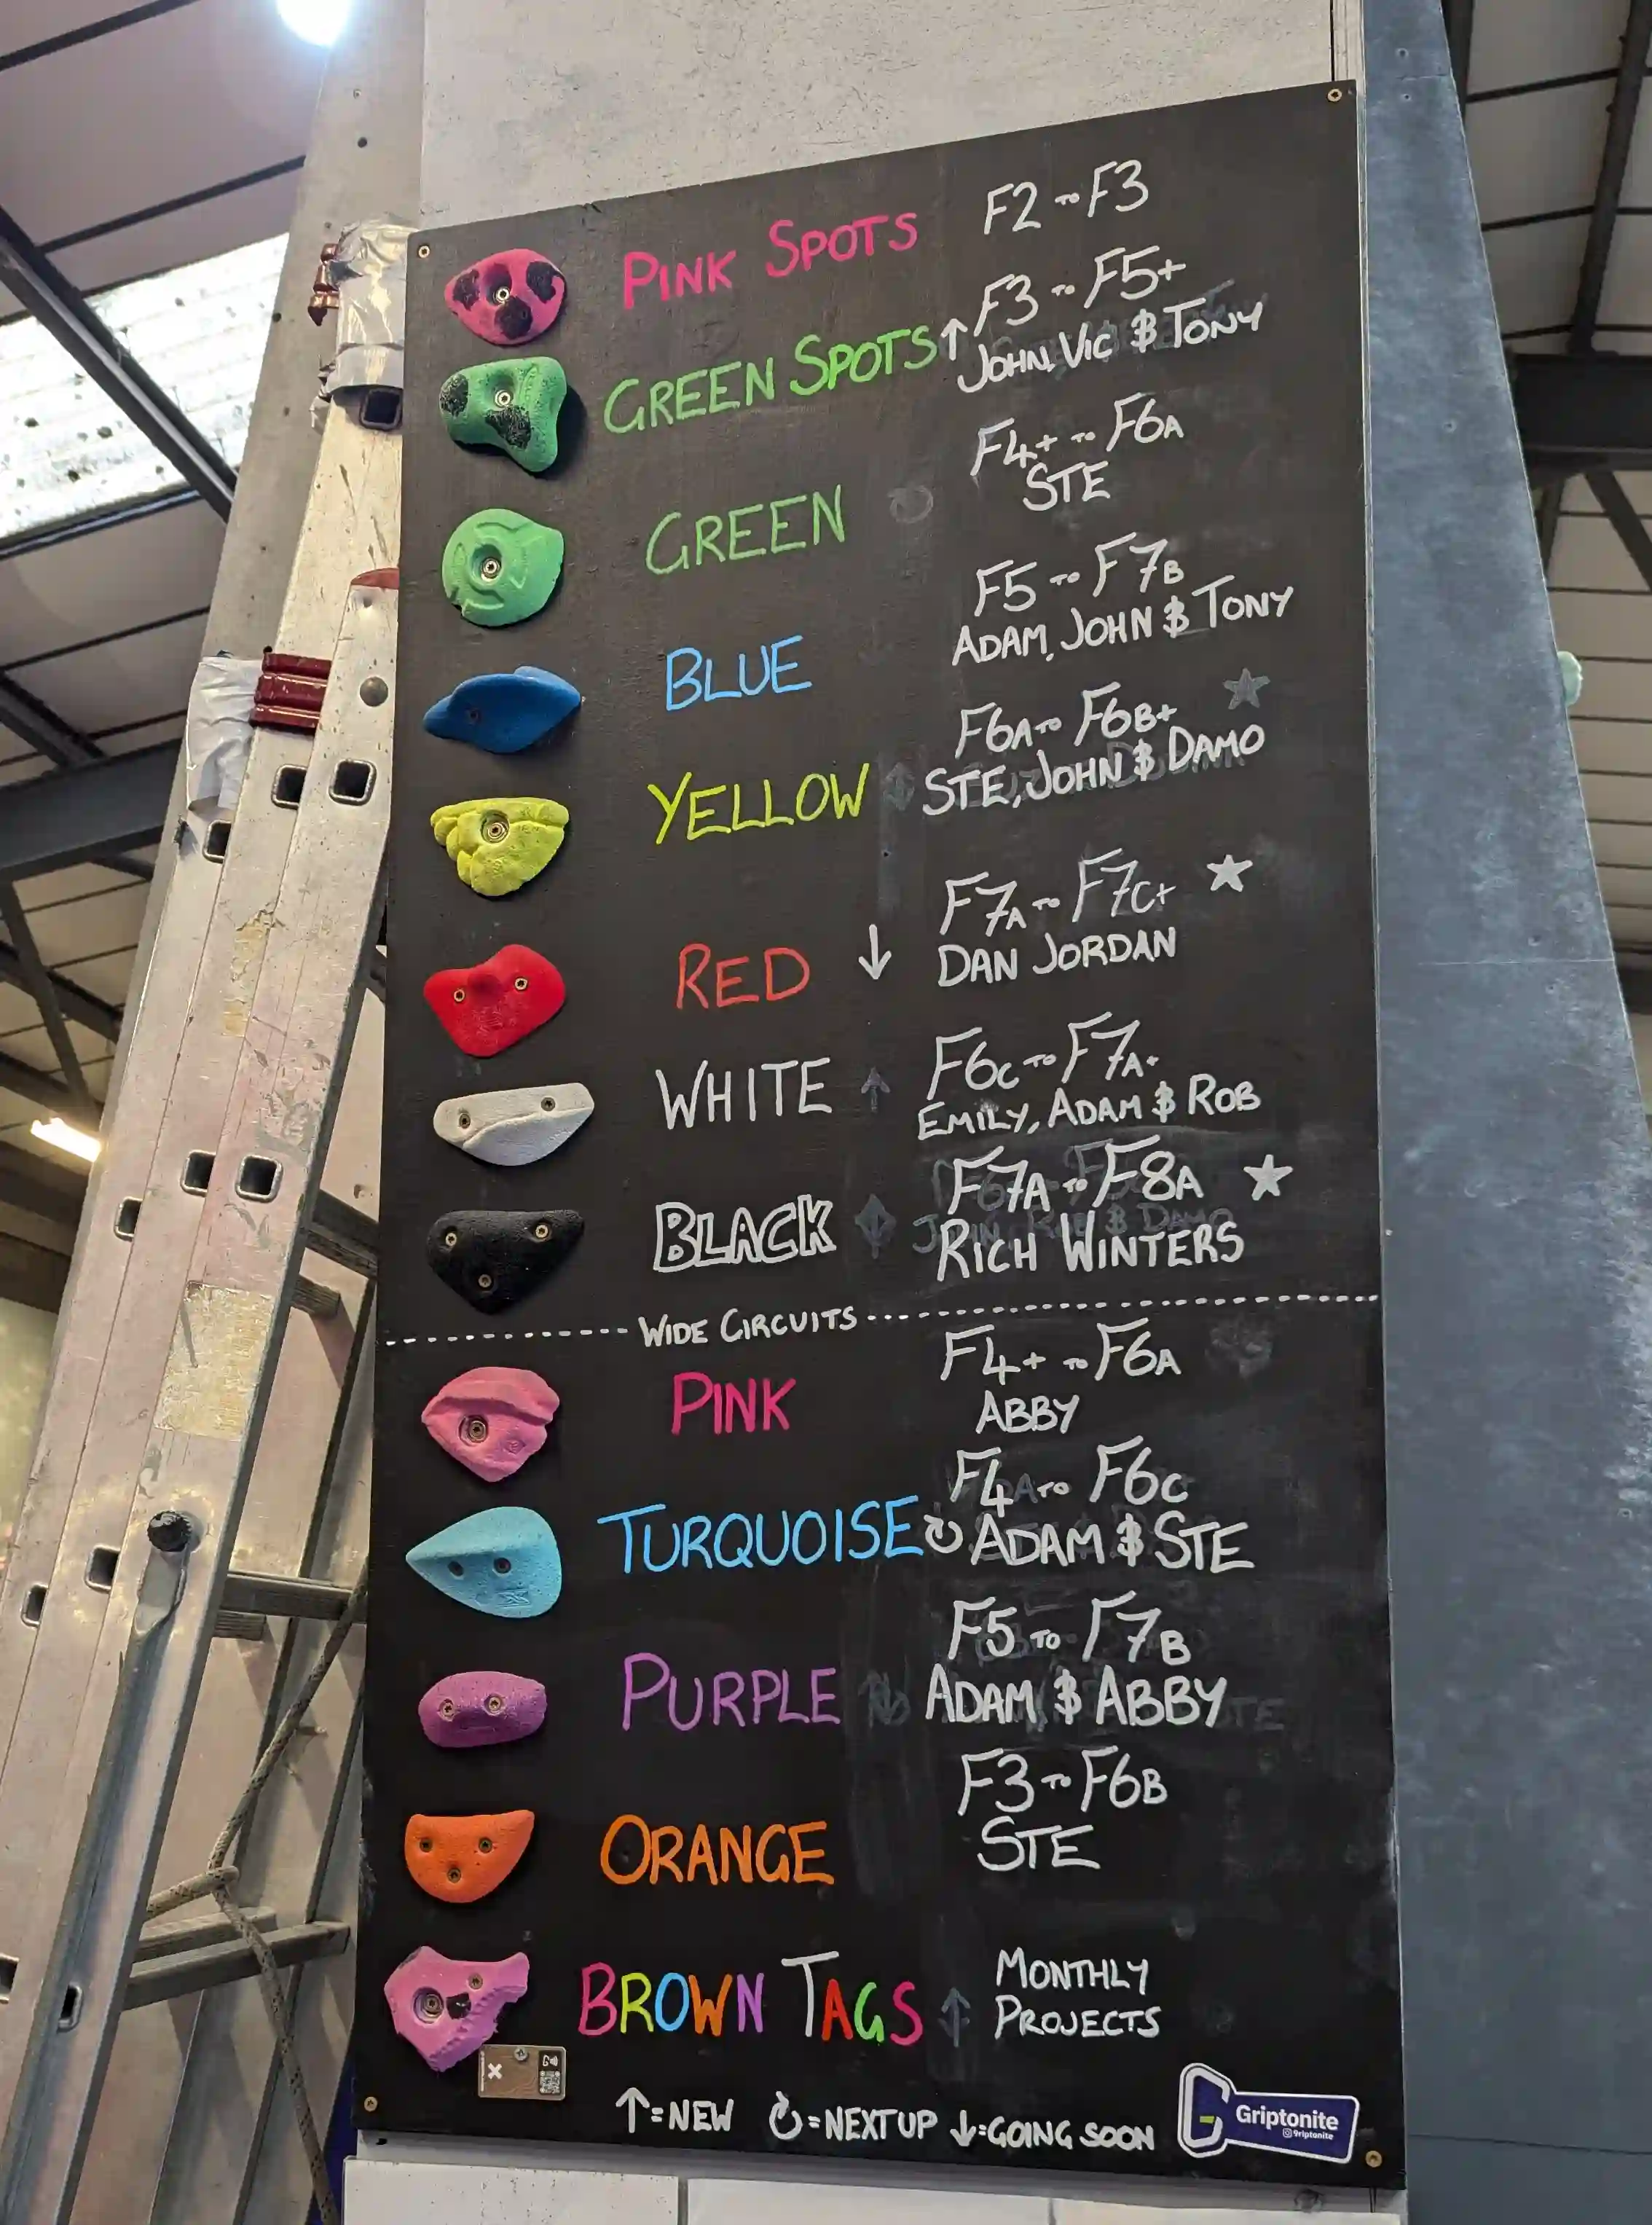
\includegraphics[width=0.30\linewidth]{../../references/charts/chart_04_sportrock.png}}{\fbox{\parbox[c][3cm]{0.28\linewidth}{\centering Sportrock\\(\texttt{chart\_04\_sportrock.png})}}} &
\IfFileExists{../../references/charts/chart_05_rockfish.png}{
\includegraphics[width=0.30\linewidth]{../../references/charts/chart_05_rockfish.png}}{\fbox{\parbox[c][3cm]{0.28\linewidth}{\centering Rockfish Climbing\\(\texttt{chart\_05\_rockfish.png})}}} &
\IfFileExists{../../references/charts/chart_06_j2_bouldering.jpg}{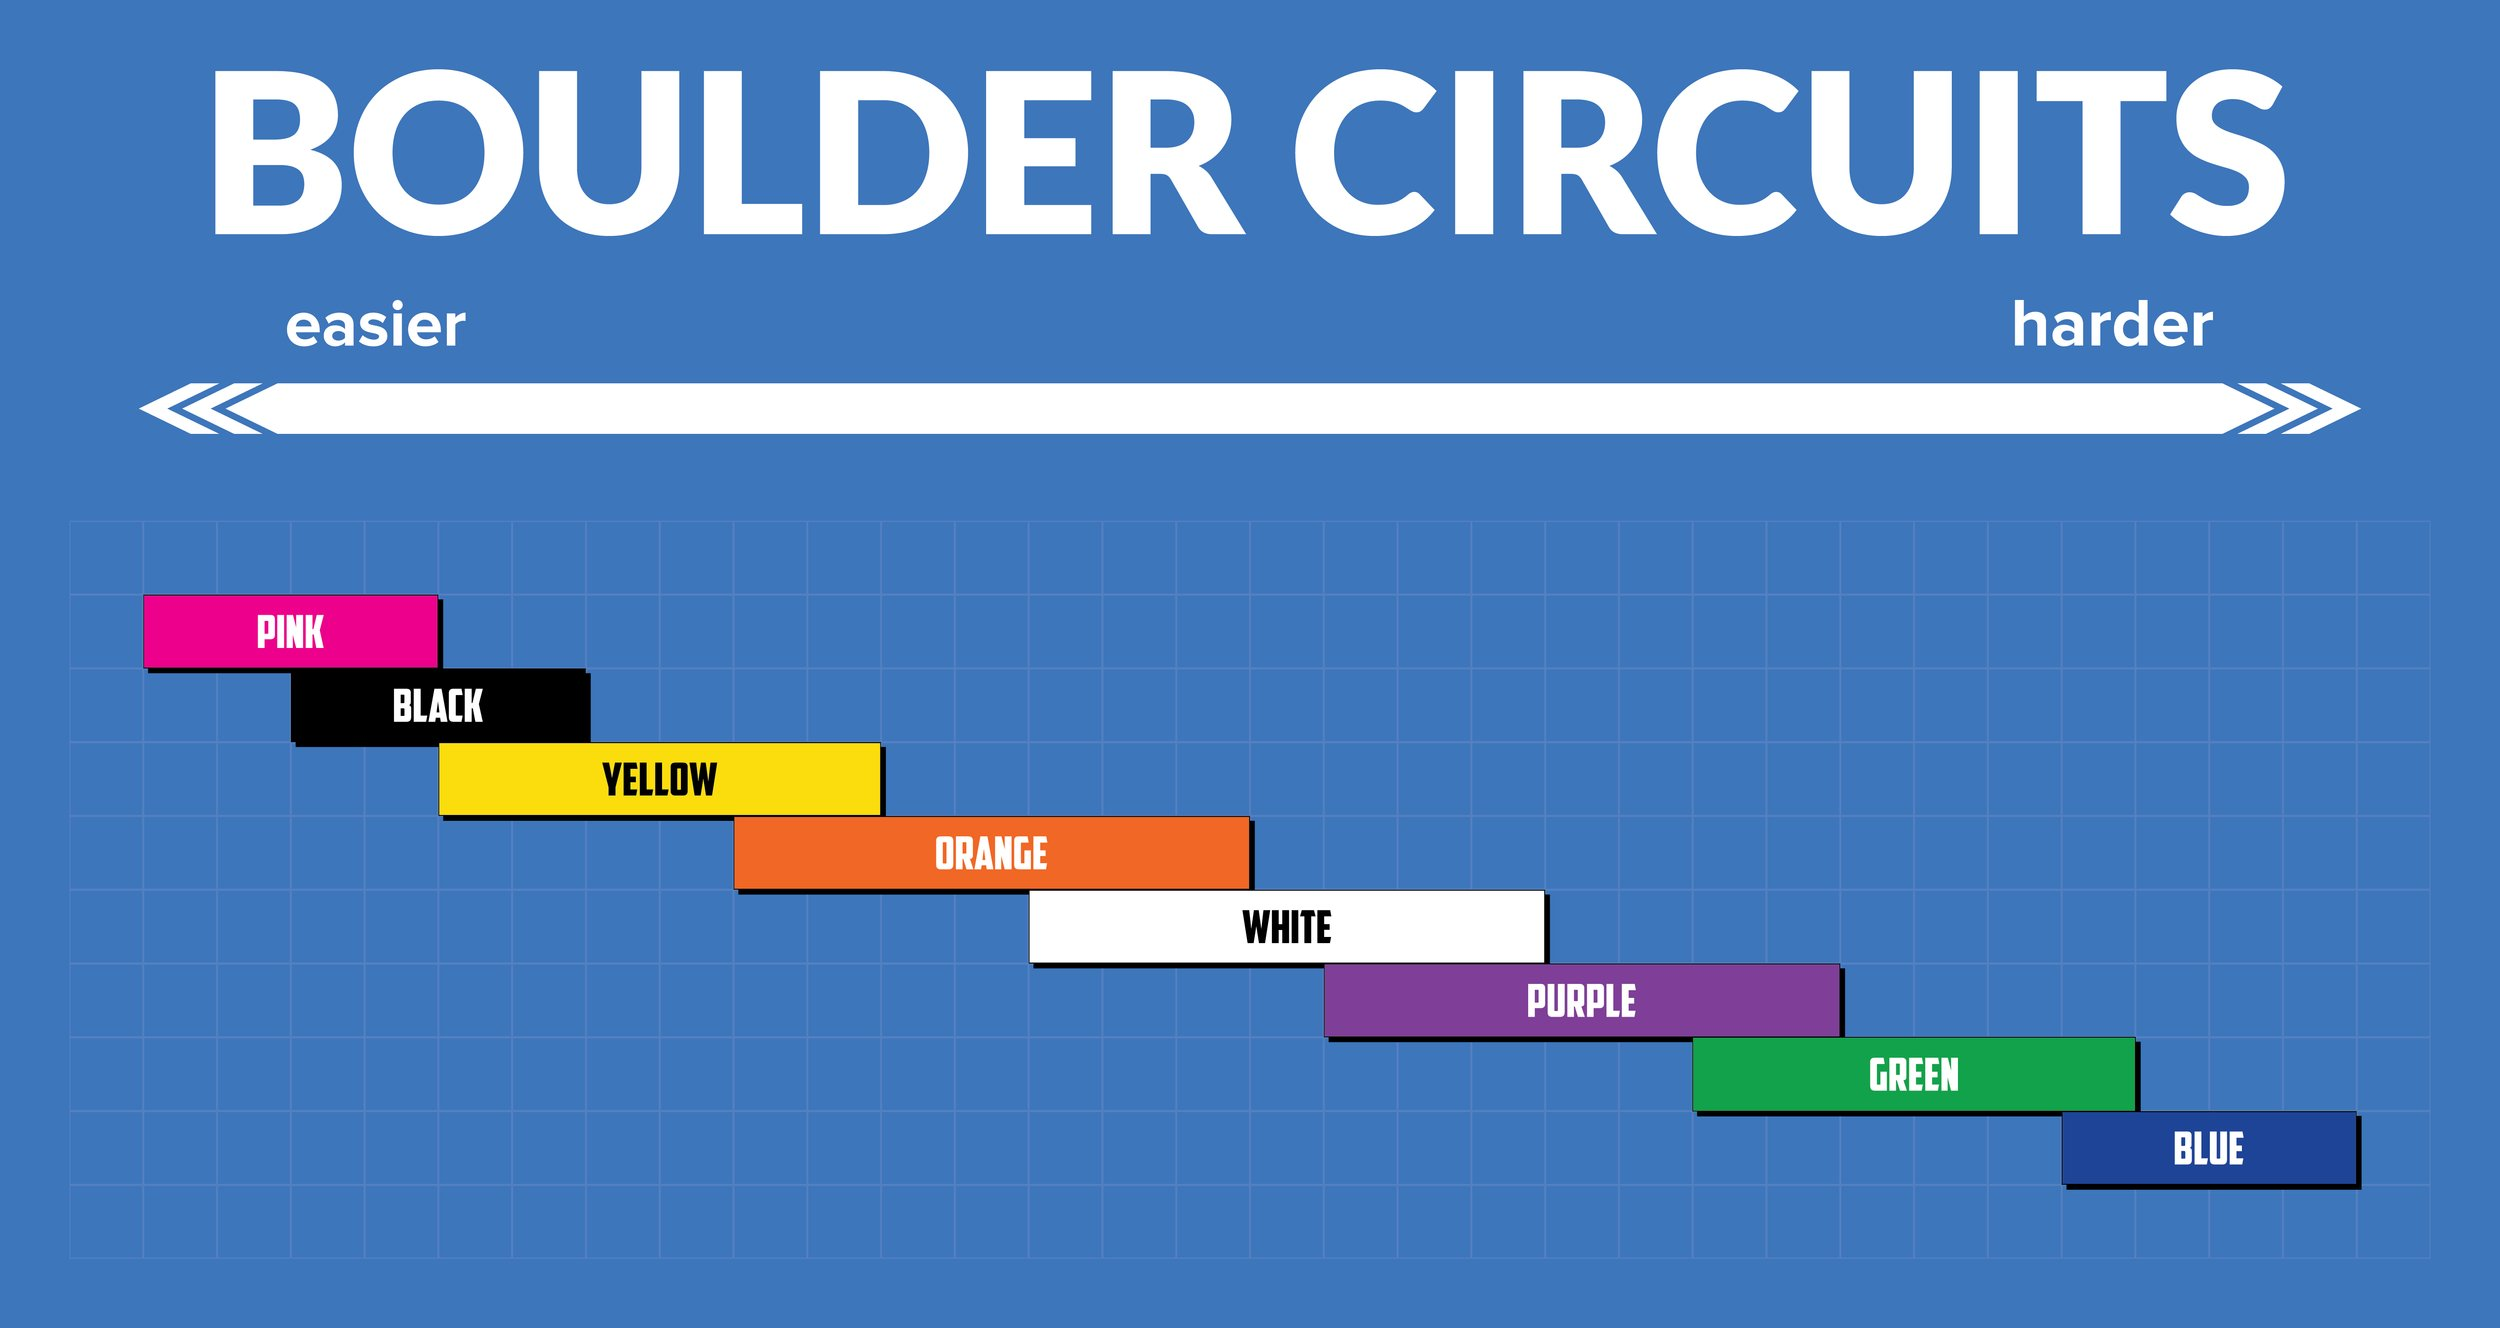
\includegraphics[width=0.30\linewidth]{../../references/charts/chart_06_j2_bouldering.jpg}}{\fbox{\parbox[c][3cm]{0.28\linewidth}{\centering J2 Bouldering\\(\texttt{chart\_06\_j2\_bouldering.jpg})}}} \\[4pt]
(d) Sportrock & (e) Rockfish Climbing & (f) J2 Bouldering
\end{tabular}
\end{figure}

\noindent\textit{Síntese:} Circuitos por fitas ou etiquetas resolvem a restrição de estoque de agarras, enquanto faixas sobrepostas de dois graus (com proteção explícita da base VB--V0) garantem progressão contínua e comparável entre ginásios.


\clearpage
% EDITORIAL QUESTION: Como correlacionar de forma unificada as escalas internacionais e estruturar uma matriz cromática de nove faixas protegendo a iniciação?
\section{Matrizes de Equivalência Internacional e Referência de Circuitos}

Esta seção apresenta a \textbf{Tabela~\ref{tab:equivalencia_mestra}} (Matriz Mestra de Equivalência Internacional com foco estrito em boulder e lance-crux) e a \textbf{Tabela~\ref{tab:circuitos_referencia}} (Matriz de Referência de Nove Faixas Cromáticas).

\begin{table}[!htbp]
\centering
\caption{Matriz Mestra de Equivalência Internacional (Foco em Boulder e Lance-Crux).}
\label{tab:equivalencia_mestra}
\footnotesize
\renewcommand{\arraystretch}{1.15}
\begin{tabularx}{\linewidth}{ccccccX}
\toprule
\textbf{IRCRA} & \textbf{V-Scale} & \textbf{FB} & \textbf{CBME} & \textbf{YDS} & \textbf{Ewbank} & \textbf{Exigência Biomecânica e Perfil Motor Típico} \\
\midrule
\textbf{8}  & —   & 4-  & IV    & 5.8   & 14 & Iniciação absoluta; subida tipo escada em jarros (\textit{jugs}) amplos e simétricos. \\
\rowcolor{rowgray}
\textbf{9}  & \textbf{VB}  & 4   & V     & 5.9   & 15 & Base motora elementar; transferência de peso sobre pés grandes sem força isolada de dedos. \\
\textbf{11} & \textbf{V0-} & 4+  & VI    & 5.10b & 17 & Consciência de quadril próximo à parede; bordas positivas largas e pés direcionais. \\
\rowcolor{rowgray}
\textbf{12} & \textbf{V0}  & 5   & VI    & 5.10c & 18 & Equilíbrio espacial; agarras oblíquas positivas, oposição e trocas de pé precisas. \\
\textbf{13} & \textbf{V0+} & 5+  & VIsup & 5.10d & 19 & Transição intermediária; negativos leves ou placas técnicas com apoios de pé reduzidos. \\
\rowcolor{rowgray}
\textbf{14} & \textbf{V1}  & 6A  & VIIa  & 5.11a & 20 & Força isométrica nos flexores dos dedos; bordas retas, pinças médias e leitura de sequência. \\
\textbf{15} & \textbf{V2}  & 6A+ & VIIb  & 5.11b & 21 & Ganchos de calcanhar (\textit{heel hook}), bandeiras (\textit{flagging}) e pequenos botes. \\
\rowcolor{rowgray}
\textbf{16} & \textbf{V3}  & 6B  & VIIc  & 5.11c & 22 & Negativos moderados e placas exigentes; cruzamentos sob tensão, abaulados e compressão. \\
\rowcolor{rowgray}
\textbf{17} & \textbf{V3+} & 6B+ & VIIc  & 5.11d & 23 & Sequências contínuas de 5 a 8 movimentos intensos sem descanso intermediário. \\
\rowcolor{rowgray}
\textbf{18} & \textbf{V4}  & 6C  & VIIIa & 5.12a & 24 & Nível avançado inicial; regletes de 15--20\,mm, tensão de tronco e bloqueios altos. \\
\textbf{19} & \textbf{V5}  & 6C+ & VIIIb & 5.12b & 25 & Bloqueios unilaterais profundos, \textit{toe hooks} em tetos e dinâmicos longos. \\
\rowcolor{rowgray}
\textbf{20} & \textbf{V6}  & 7A  & VIIIc & 5.12c & 26 & Alto desempenho; coordenação dinâmica complexa, regletes vivos e compressão em volumes. \\
\textbf{21} & \textbf{V7}  & 7A+ & IXa   & 5.12d & 27 & Nível expert; regletes mínimos ($\le 12$\,mm) e alta taxa de produção de força (RFD). \\
\rowcolor{rowgray}
\textbf{22} & \textbf{V8}  & 7B  & IXb   & 5.13a & 28 & Alta performance competitiva; força digital extrema, mobilidade de quadril e precisão. \\
\rowcolor{rowgray}
\textbf{24} & \textbf{V9}  & 7C  & IXc   & 5.13c & 29 & Entrada na elite esportiva; alta intensidade sustentada sem margem para ajuste postural. \\
\rowcolor{rowgray}
\textbf{26} & \textbf{V10} & 7C+ & Xb    & 5.14a & 31 & Padrão de finais nacionais/internacionais e projetos clássicos em rocha natural. \\
\bottomrule
\end{tabularx}
\end{table}

\clearpage
\subsection*{3.1 Matriz de Referência de Circuitos (Nove Faixas Cromáticas)}

% SOURCE [INTERPRETATION]: Síntese aplicada das equivalências IRCRA (Draper et al., 2016) e CBME DT-2016/01 com divisão da faixa de entrada em Branco-Vazado e Branco.
\begin{table}[!htbp]
\centering
\caption{Matriz de Referência de Circuitos por Cores (Nove Faixas) e Equivalência Multissistêmica.}
\label{tab:circuitos_referencia}
\scriptsize
\renewcommand{\arraystretch}{1.15}
\begin{tabularx}{\linewidth}{p{2.55cm}ccccp{1.8cm}X}
\toprule
\textbf{Circuito / Cor} & \textbf{V-Scale} & \textbf{FB} & \textbf{IRCRA} & \textbf{CBME} & \textbf{RIC} & \textbf{Padrão Motor e Referência Prática} \\
\midrule
\colorbox{tagwhitehollow}{\strut\color{black}\textbf{0. Branco-Vazado}} & \textbf{VB / V0} & 4--5 & 8--12 & IV--VI & \texttt{R1 I1 C1} & \textbf{Iniciação Absoluta}: Agarras anatômicas francas (\textit{jugs}), movimento tipo escada em parede positiva ou vertical. \\
\rowcolor{rowgray}
\colorbox{tagwhite}{\strut\color{black}\textbf{1. Branco}} & \textbf{V0 / V1} & 5--6A & 12--14 & VI--VIIa & \texttt{R1 I1-2 C1-2} & \textbf{Transição Básica}: Introdução a bordas positivas, equilíbrio espacial e primeiros passos de oposição. \\
\colorbox{tagyellow}{\strut\color{black}\textbf{2. Amarela}} & \textbf{V1 / V2} & 6A--6A+ & 14--15 & VIIa/b & \texttt{R1-2 I2 C2} & \textbf{Iniciante Consolidado}: Centro de gravidade, pés precisos, primeiros \textit{heel hooks} e posicionamento lateral. \\
\rowcolor{rowgray}
\colorbox{taggreen}{\strut\color{white}\textbf{3. Verde}} & \textbf{V2 / V3} & 6A+--6B+ & 15--17 & VIIb/c & \texttt{R2 I2-3 C2-3} & \textbf{Intermediário}: Negativos moderados, placas em ponta de pé, pinças e cruzamentos controlados. \\
\colorbox{tagblue}{\strut\color{white}\textbf{4. Azul}} & \textbf{V3 / V4} & 6B--6C & 16--18 & VIIc/VIIIa & \texttt{R2-3 I3 C3} & \textbf{Intermediário-Avançado}: Compressão em volumes, regletes médios (18--22\,mm) e tensão abdominal. \\
\rowcolor{rowgray}
\colorbox{tagred}{\strut\color{white}\textbf{5. Vermelha}} & \textbf{V4 / V5} & 6C--6C+ & 18--19 & VIIIa/b & \texttt{R3 I3-4 C3-4} & \textbf{Avançado}: Bloqueios pronunciados (\textit{lock-offs}), saídas de teto e botes de coordenação. \\
\colorbox{tagblack}{\strut\color{white}\textbf{6. Preta}} & \textbf{V5 / V6} & 6C+--7A & 19--20 & VIIIb/c & \texttt{R3-4 I4 C4} & \textbf{Avançado Consolidado}: Patamar de Font 7A; regletes incisivos (12--15\,mm) e compressão ampla. \\
\rowcolor{rowgray}
\colorbox{tagsilver}{\strut\color{black}\textbf{7. Prata}} & \textbf{V6 / V7} & 7A--7A+ & 20--21 & VIIIc/IXa & \texttt{R4 I4-5 C4} & \textbf{Alto Rendimento}: Baixa margem de erro, força isométrica elevada e coordenação tridimensional. \\
\colorbox{taggold}{\strut\color{black}\textbf{8. Dourada}} & \textbf{V7 / V8+} & $\ge$ 7A+/7B & $\ge$ 21--22 & $\ge$ IXa/b & \texttt{R4-5 I5 C5} & \textbf{Elite Nacional}: Limite biomecânico do ginásio; regletes milimétricos e saltos duplos de competição. \\
\bottomrule
\end{tabularx}
\end{table}

\noindent\textit{Síntese:} A divisão da entrada em \textbf{Branco-Vazado} (VB/V0) e \textbf{Branco} (V0/V1) elimina o salto de cinco degraus IRCRA em uma única cor, preservando a sobreposição gradual a partir do circuito Amarelo.


\clearpage
\section*{Conclusão e Diretrizes Operacionais}
\addcontentsline{toc}{section}{Conclusão e Diretrizes Operacionais}

A revisão bibliográfica demonstra que a graduação em escalada não é um juízo arbitrário, mas um sistema multidimensional controlável. Cinco diretrizes operacionais sintetizam a aplicação prática para qualquer ginásio brasileiro:

\begin{enumerate}
    \item \textbf{Vias-Gabarito (\textit{Benchmark Boulders})}: Manter de 8 a 12 blocos de referência calibrados com polos de rocha nacional (Cocalzinho e Igatu) para ancorar os circuitos.
    \item \textbf{Forerunning Obrigatório}: Proibir a graduação por um único \textit{setter}, exigindo validação por testadores de estaturas distintas para eliminar viés morfológico e \textit{beta breaks} \cite{cwa_setting, anderson_routesetting}.
    \item \textbf{Proteção da Base}: Separar a iniciação absoluta (\texttt{VB/V0}) da transição (\texttt{V0/V1}) por meio de faixas distintas ou sub-identificadores claros na base da via \cite{ircra_draper, cwa_setting}.
    \item \textbf{Governança Híbrida}: Combinar parede física limpa (fitas/tags) com registro unitário em aplicativo digital, auditando divergências superiores a 1 grau após 15 repetições \cite{topclimbing_platform, pmc_ric_study}.
    \item \textbf{Vínculo Institucional}: Cadastrar o ginásio no SGE da CBEscalada para habilitar atletas vinculados ao calendário oficial e programas de fomento \cite{cbescalada_filiacoes}.
\end{enumerate}


\appendix
\clearpage
% EDITORIAL QUESTION: Como evoluíram historicamente as escalas de graduação na Europa, EUA e Brasil até os polos modernos de referência?
\section{Evolução Histórico-Geográfica das Escalas}

Os sistemas atuais resultam de um século de transição entre escalas fechadas e abertas.

\subsection*{A.1 Das Escalas Alpinas Fechadas à Abertura de Yosemite e da UIAA}
% SOURCE [VERIFIED_PRIMARY]: UIAA History (https://www.theuiaa.org/inside-the-uiaa/history/); Sportrock (https://www.sportrock.com/post/understanding-climbing-grades).
Em \textbf{1926}, Willo Welzenbach propôs nos Alpes uma escala fechada de Grau I a Grau VI \cite{uiaa_history}. Em \textbf{1935}, o Sierra Club criou o \textbf{Sistema Decimal de Yosemite (YDS)}, dividindo a montanha em cinco classes e prevendo a Classe 5 fechada entre \texttt{5.0} e \texttt{5.9}. A evolução técnica em Yosemite forçou a abertura para \texttt{5.10a--d} até \texttt{5.15d}, e a UIAA aboliu o teto do Grau VI em 1978 \cite{uiaa_history, sportrock_grades}.

\subsection*{A.2 Fontainebleau: Circuitos por Cores e Escala Font}
% SOURCE [VERIFIED_PRIMARY]: Climb Ski Boulder Magazine; BMC Grades (https://thebmc.co.uk/en/indoor-climbing-grades-explained).
Em \textbf{1947}, Fred Bernuz pintou em Fontainebleau o primeiro circuito numerado por cores (\textit{Amarelo, Laranja, Azul, Vermelho, Preto e Branco}), originando os circuitos comerciais modernos \cite{climbski_font, arkose_niveaux}. Paralelamente, consolidou-se a escala alfanumérica \textit{Font} com letras maiúsculas a partir do sexto grau (\texttt{6A} a \texttt{9A}) para distingui-la das vias de corda francesas (\texttt{6a}, \texttt{7b+}) \cite{bmc_grades, actugrimpe_niveaux}.

\subsection*{A.3 John Gill (Escala B) e John Sherman (Escala V)}
% SOURCE [VERIFIED_PRIMARY]: Sherman (1991), Hueco Tanks Guide; Movement Gyms (https://blog.movementgyms.com/understanding-v-grades).
Nos anos 1950, John Gill introduziu o magnésio e a \textbf{Escala B} (\textit{B1, B2, B3}) \cite{movement_vgrades}. Em \textbf{1991}, no guia de Hueco Tanks, John ``Vermin'' Sherman sistematizou a \textbf{Escala Hueco ($V$-Scale)} a partir de $V0$ (posteriormente expandida de \textbf{VB} até \textbf{V17}), hoje padrão nas Américas, África do Sul e Oceania \cite{sherman_hueco, cityrock_guide}.

\begin{table}[!htbp]
\centering
\caption{Síntese histórico-geográfica dos principais sistemas de graduação.}
\label{tab:sistemas_mundo}
\footnotesize
\renewcommand{\arraystretch}{1.12}
\begin{tabularx}{\linewidth}{p{2.2cm}p{2.3cm}p{2.4cm}X}
\toprule
\textbf{Sistema} & \textbf{Origem / Ano} & \textbf{Notação Típica} & \textbf{Escopo e Lógica Estrutural} \\
\midrule
\textbf{UIAA} & Alpes / 1926--1947 & \texttt{V+, VI, VII-, IX+} & Escala em romanos; aberta acima do Grau VI em 1978 \cite{uiaa_history}. \\
\rowcolor{rowgray}
\textbf{Fontainebleau} & França / anos 1940 & \texttt{4, 5+, 6A+, 7B, 8C} & Escala aberta de boulder; letras maiúsculas (\texttt{A, B, C}) a partir do 6 \cite{bmc_grades}. \\
\textbf{YDS} & EUA / 1935--anos 50 & \texttt{5.9, 5.10c, 5.12a} & Sistema decimal de Yosemite; subdividido em \texttt{a--d} a partir de \texttt{5.10} \cite{sportrock_grades}. \\
\rowcolor{rowgray}
\textbf{Ewbank} & Austrália / África do Sul (1967) & \texttt{14, 18, 22, 28, 35} & Escala aberta estritamente numérica contínua para vias \cite{cityrock_guide}. \\
\textbf{Hueco ($V$)} & Texas, EUA / 1991 & \texttt{VB, V0, V3, V8, V17} & Escala aberta padrão para boulder nas Américas \cite{sherman_hueco}. \\
\rowcolor{rowgray}
\textbf{CBME} & Brasil / 2007--2016 & \texttt{5º VIIa E2} / \texttt{VIIb} & Norma DT-2016/01: Grau geral arábico + Crux romano \cite{cbme_dt01}. \\
\bottomrule
\end{tabularx}
\end{table}

\subsection*{A.4 Polos Geográficos Balizadores: Cocalzinho, Igatu e Rocklands}
% SOURCE [VERIFIED_PRIMARY]: Guia de Igatu (EENe, 2014); Climber Codex Pireneus; Guia OuroBoulder (2019); CityROCK (2020).
\begin{itemize}
    \item \textbf{Cocalzinho de Goiás (GO)}: Quartzito compacto de regletes definidos e \textit{mantles} técnicos; referência nacional contra inflação de graus indoor \cite{guia_cocalzinho, guia_ouroboulder}.
    \item \textbf{Vila de Igatu (BA)}: Quartzito áspero de formação tridimensional na Chapada Diamantina, exigindo compressão e pinças em tetos \cite{guia_igatu}.
    \item \textbf{Rocklands (África do Sul)}: Referência global em arenito quartzítico para validação da Escala $V$, espelhada nos ginásios da Cidade do Cabo \cite{cityrock_guide, goodbeta_sa}.
\end{itemize}


\clearpage
% EDITORIAL QUESTION: Como comparar metodologicamente as escalas IRCRA e RIC e por que não existem benchmarks físicos universais isolados para valores pontuais?
\section{Escalas IRCRA, RIC e Limites do Método Científico}

\subsection*{B.1 Comparação Estrutural: IRCRA vs. RIC}
% SOURCE [VERIFIED_PRIMARY]: Draper et al. (2016); PMC11881084 (2024) (https://pmc.ncbi.nlm.nih.gov/articles/PMC11881084/).
Embora frequentemente citadas juntas em estudos recentes, \textbf{IRCRA} e \textbf{RIC} medem grandezas ortogonais:
\begin{itemize}
    \item \textbf{IRCRA (\textit{Reporting Scale})}: Escala ordinal/quase-linear unidimensional (valores inteiros de 1 a 32/39) desenhada para agregar dados estatísticos de dificuldade entre escalas alfanuméricas heterogêneas \cite{ircra_draper, pmc_ric_study}.
    \item \textbf{RIC (\textit{Risk, Intensity, Complexity})}: Vetor tridimensional intra-grau (métricas de 1 a 5) usado por equipes de \textit{setters} para decompor o perfil qualitativo de um problema dentro de um mesmo grau nominal \cite{pmc_ric_study, godoffe_routesetting}.
\end{itemize}

\subsection*{B.2 Ausência de Padrão Físico Universal Isolado vs. Painéis Padronizados}
% SOURCE [VERIFIED_PRIMARY]: PMC11881084 (2024); Rock Climbing Realms (2025) (https://rockclimbingrealms.com/the-setters-secret-how-gym-climb-grades-emerge/).
Uma questão metodológica central é se existem testes físicos universais que fixem isoladamente valores como ``IRCRA 10'' ou ``$I = 2$'' na escala RIC. A revisão da literatura (\cite{pmc_ric_study, rockrealms_setting}) confirma que \textbf{não existe padrão físico universal isolado independente de contexto}:
\begin{enumerate}
    \item O valor $I = 2$ na RIC é estritamente \textbf{relativo} ao público e ao consenso da equipe de \textit{setting} local, servindo para balancear variedade intra-grau, e não como unidade absoluta de força em newtons \cite{pmc_ric_study}.
    \item Na prática empírica e em modelos de aprendizado de máquina, a única padronização física transnacional de referência ocorre por meio de \textbf{placas de treino com geometria e agarras fixas} — como o \textbf{MoonBoard} (grade fixa de 198 posições com mais de 30.000 problemas registrados) e o \textbf{Kilter Board} — onde o consenso de milhares de repetições calibra o grau sobre um \textit{hardware} invariante \cite{pmc_ric_study, rockrealms_setting}.
    \item Testes laboratoriais isolados (como suspensão máxima em reglete de 20\,mm) correlacionam-se estatisticamente com o nível IRCRA do atleta, mas não determinam sozinhos o grau de uma via por omitirem complexidade motora ($C$) e risco ($R$) \cite{rpubs_finger, pmc_ric_study}.
\end{enumerate}


\clearpage
% EDITORIAL QUESTION: Quais definições operacionais padronizam a comunicação entre setters, gestores e praticantes?
\section{Glossário Técnico e Termos Operacionais}

\begin{description}
    \item[Beta / Beta Break:] Sequência de movimentos planejada pelo \textit{setter} para resolver um bloco; \textit{beta break} ocorre quando o escalador encontra solução alternativa não prevista que reduz a dificuldade pretendida.
    \item[Conquistador / Abertura de Via:] Termos reservados neste documento exclusivamente para a escalada em rocha natural (conforme ética da CBME DT-2016/10).
    \item[Crux:] Lance ou sequência de movimentos mais difícil de uma via ou boulder.
    \item[Forerunning:] Processo coletivo de testagem prévia de blocos recém-montados por múltiplos \textit{setters} de estaturas distintas antes da liberação ao público.
    \item[Grau Trabalhado (``Decotar''):] Execução após ensaio prévio dos movimentos (\textit{redpoint}), em contraste com a escalada \textit{à vista} (\textit{onsight}) exigida como referência na CBME DT-2016/01.
    \item[Setter (ou Routesetter):] Profissional ou membro técnico responsável por projetar, montar e calibrar percursos em muros artificiais.
    \item[Start Tag:] Etiqueta fixada na agarra de largada contendo circuito, cor, metadados e subgrau.
\end{description}


\clearpage
\begin{thebibliography}{99}

\bibitem{cbme_dt01}
Confederação Brasileira de Montanhismo e Escalada (CBME).
\newblock \textit{Diretriz Técnica CBME DT-2016/01: Sistema Brasileiro de Graduação de Vias de Escalada}.
\newblock Rio de Janeiro: CBME, 03 dez. 2016, 14 págs. Disponível em: \url{https://cbme.org.br/novo/wp-content/uploads/2025/03/CBME-DT-2016_01-Sistema-Brasileiro-de-graduacao-de-vias-de-escalada.pdf}.

\bibitem{cbme_dt10}
Confederação Brasileira de Montanhismo e Escalada (CBME).
\newblock \textit{Diretriz Técnica CBME DT-2016/10: Padrões Éticos e Diretrizes para Conquista e Equipagem de Vias}.
\newblock Rio de Janeiro: CBME, 2016. Disponível em: \url{http://www.cbme.org.br/novo/wp-content/uploads/2017/01/CBME_DT_2016_10-1.pdf}.

\bibitem{cbescalada_sobre}
Confederação Brasileira de Escalada Esportiva (CBEscalada).
\newblock \textit{Institucional: História, Reconhecimento COB/CPB e Centro de Treinamento}.
\newblock CBEscalada, 2026. Disponível em: \url{https://cbescalada.org.br/entidade/9/sobre}.

\bibitem{cbescalada_filiacoes}
Confederação Brasileira de Escalada Esportiva (CBEscalada).
\newblock \textit{Regulamento de Filiações 2026: SGE, Bolsa Atleta e Cadastro de Ginásios}.
\newblock CBEscalada, 2026. Disponível em: \url{https://cbescalada.org.br/atletas/74/filiacoes}.

\bibitem{worldclimbing_about}
World Climbing (antiga IFSC).
\newblock \textit{About World Climbing: Institutional History and Olympic/Paralympic Recognition}.
\newblock Turim, 2025/2026. Disponível em: \url{https://www.worldclimbing.com/ifsc}.

\bibitem{worldclimbing_rebrand}
World Climbing.
\newblock \textit{World Climbing Launches New Global Identity and World Climbing Series}.
\newblock 10 dez. 2025. Disponível em: \url{https://www.worldclimbing.com/news/world-climbing-launches-new-global-identity}.

\bibitem{ifsc_rules}
World Climbing / IFSC.
\newblock \textit{IFSC Rules 2025 \& Route Setters Commission Technical Regulations}.
\newblock Disponível em: \url{https://www.worldclimbing.com/commissions/routesetters}.

\bibitem{ifsc_paraclimbing}
World Climbing / IFSC.
\newblock \textit{Paraclimbing Classification Rules and Routesetting Guidelines}.
\newblock Disponível em: \url{https://images.ifsc-climbing.org/ifsc/image/private/t_q_good/prd/upkzmyetexs1g63fzxyd.pdf}.

\bibitem{uiaa_history}
UIAA.
\newblock \textit{History of the UIAA and Evolution of Alpine Grading Systems}.
\newblock Berna, 2024. Disponível em: \url{https://www.theuiaa.org/inside-the-uiaa/history/}.

\bibitem{ircra_draper}
Draper, N. et al.
\newblock Reporting grades in rock climbing: a position statement.
\newblock \textit{Sports Technology}, v.~8, n.~3--4, págs.~85--93, 2015/2016. Disponível em: \url{https://ircra.rocks/reporting-grades-in-climbing-research/}.

\bibitem{pmc_ric_study}
National Institutes of Health (NIH) / PubMed Central.
\newblock \textit{Addressing grading bias in rock climbing: machine and deep learning approaches and the RIC framework}.
\newblock PMC11881084, 2024/2025. Disponível em: \url{https://pmc.ncbi.nlm.nih.gov/articles/PMC11881084/}.

\bibitem{godoffe_routesetting}
Godoffe, J. \& Katiyo, T.
\newblock \textit{My Keys to Routesetting / The Art of Routesetting}.
\newblock Paris, 2017.

\bibitem{anderson_routesetting}
Anderson, L.
\newblock \textit{Fundamentals of Routesetting}.
\newblock Guilford, CT: Falcon Guides, 2014.

\bibitem{cwa_setting}
Climbing Wall Association (CWA).
\newblock \textit{How to Routeset \& Grade Routes in Gyms Far From Outdoor Climbing}.
\newblock CWA Pro Blog, 2023. Disponível em: \url{https://www.cwapro.org/blog/how-to-routeset-and-grade-routes-in-gyms-far-from-outdoor-climbing}.

\bibitem{cwa_colors}
Climbing Wall Association (CWA).
\newblock \textit{How Do You Decide What Colors To Set Your Walls?}.
\newblock CWA Pro Blog, 2022. Disponível em: \url{https://www.cwapro.org/blog/how-do-you-decide-what-colors-to-set-your-walls}.

\bibitem{cbj_tape}
Climbing Business Journal (CBJ).
\newblock \textit{Tape to No Tape in 6 Steps}.
\newblock CBJ, 2019/2023. Disponível em: \url{https://climbingbusinessjournal.com/tape-to-no-tape-in-6-steps/}.

\bibitem{bmc_grades}
British Mountaineering Council (BMC).
\newblock \textit{Indoor Climbing Grades Explained}.
\newblock BMC, 2023. Disponível em: \url{https://thebmc.co.uk/en/indoor-climbing-grades-explained}.

\bibitem{bp_grades}
Bouldering Project (BP).
\newblock \textit{How to Understand Climbing Grades at Any Gym}.
\newblock 2023. Disponível em: \url{https://boulderingproject.com/blog/understand-climbing-grades-at-any-gym/}.

\bibitem{gearloop_tempe}
GearLoop.
\newblock \textit{Bouldering Project Tempe \& Brooklyn Grading Boards}.
\newblock 2024. Disponível em: \url{https://gearloop.app/gyms/bouldering-project-tempe/}.

\bibitem{arkose_niveaux}
Arkose.
\newblock \textit{Niveau escalade \& bloc couleur}.
\newblock Paris, 2024. Disponível em: \url{https://arkose.com/groupe/actus/niveau-escalade-bloc-couleur-tout-comprendre}.

\bibitem{cityrock_guide}
CityROCK South Africa.
\newblock \textit{How to Climb at CityROCK: Grading Conversion Chart}.
\newblock 2020. Disponível em: \url{https://cityrock.co.za/HowtoClimb2020.pdf}.

\bibitem{agility_ric}
Agility Boulders.
\newblock \textit{Circuits + RIC: How We Build Meaningful Climbing Experiences}.
\newblock 2023. Disponível em: \url{https://www.agilityboulders.com/post/circuits-ric-how-we-build-meaningful-climbing-experiences}.

\bibitem{topclimbing_platform}
TopClimbing Brasil.
\newblock \textit{Plataforma Digital de Gestão para Academias de Escalada}.
\newblock 2024/2026. Disponível em: \url{https://topclimbing.com.br/}.

\bibitem{sherman_hueco}
Sherman, J.
\newblock \textit{Hueco Tanks Climbing and Bouldering Guide}.
\newblock Chockstone Press / Falcon, 1991.

\bibitem{guia_cocalzinho}
Climber Codex.
\newblock \textit{Parque Estadual dos Pireneus | Guia de Escalada de Cocalzinho de Goiás}.
\newblock Disponível em: \url{https://climbercodex.com/ptbr/routes/parque-estadual-dos-pirineus}.

\bibitem{guia_ouroboulder}
OuroBoulder.
\newblock \textit{Guia de Escalada OuroBoulder 2019}.
\newblock Disponível em: \url{https://tadejatravels.com/pdf/vodnik-GUIA-OUROBOULDER.pdf}.

\bibitem{guia_igatu}
EENe.
\newblock \textit{Guia de Escaladas de Igatu --- Chapada Diamantina, BA}.
\newblock 2014. Disponível em: \url{https://eene.com.br/wp-content/uploads/2023/03/2014_guia_igatu.pdf}.

\bibitem{youthclimbing_conv}
Youth Climbing.
\newblock \textit{Climbing Grade Converter: V-Scale, YDS, French, Font and IRCRA}.
\newblock Disponível em: \url{https://youthclimbing.com/climbing-grades/}.

\bibitem{movement_vgrades}
Movement Gyms.
\newblock \textit{Understanding V-Grades}.
\newblock Disponível em: \url{https://blog.movementgyms.com/understanding-v-grades}.

\bibitem{sportrock_grades}
Sportrock Climbing Centers.
\newblock \textit{Understanding Climbing Grades}.
\newblock Disponível em: \url{https://www.sportrock.com/post/understanding-climbing-grades}.

\bibitem{climbski_font}
Climb Ski Boulder Magazine.
\newblock \textit{Bouldering in Fontainebleau: Guide to Historical Color Circuits}.
\newblock Disponível em: \url{https://climbskibouldermagazine.com/bouldering-in-fontainebleau-guide-to-circuits-and-rock/}.

\bibitem{actugrimpe_niveaux}
ActuGrimpe.
\newblock \textit{Niveaux escalade bloc}.
\newblock Disponível em: \url{https://www.actugrimpe.com/niveaux-escalade-bloc/}.

\bibitem{paraclimbing_guide}
Paraclimbing.org.
\newblock \textit{Paraclimbing Routesetting Official Guidance}.
\newblock Disponível em: \url{https://paraclimbing.org/routesetting/}.

\bibitem{rockrealms_home}
Rock Climbing Realms.
\newblock \textit{From Random Holds to Real Routes}.
\newblock Disponível em: \url{https://rockclimbingrealms.com/setting-home-wall-routes/}.

\bibitem{rockrealms_setting}
Rock Climbing Realms.
\newblock \textit{The Setter's Secret: How Gym Climb Grades Emerge}.
\newblock Out. 2025. Disponível em: \url{https://rockclimbingrealms.com/the-setters-secret-how-gym-climb-grades-emerge/}.

\bibitem{rpubs_finger}
Yew, J.
\newblock \textit{Does Finger Strength Actually Matter in Climbing? Statistical Analysis Using the IRCRA Scale}.
\newblock RPubs, 2024. Disponível em: \url{https://rpubs.com/jyew/1470419}.

\bibitem{goodbeta_sa}
Good Beta South Africa.
\newblock \textit{South Africa Sport Climbing and Bouldering Development}.
\newblock Disponível em: \url{https://goodbeta.co.za/the-colosseum-south-africas-newest-alpine-sport-climbing-destination/}.

\bibitem{reddit_hangar}
Reddit r/bouldering \& r/indoorbouldering.
\newblock \textit{Climbing Hangar Grades \& Gym Color Schemes Survey}.
\newblock Disponível em: \url{https://www.reddit.com/r/bouldering/comments/16bp6sp/climbing_hangar_grades/}.

\bibitem{womens_gradient}
Women's Bouldering.
\newblock \textit{The Gradient of Grading: Psychological Impact of Numbers vs. Circuits}.
\newblock Disponível em: \url{https://www.womensbouldering.com/post/the-gradient-of-climbing-grading}.

\bibitem{aventura_retrato}
Aventura Alpina.
\newblock \textit{Escalada Esportiva no Brasil: O Retrato dos Atletas}.
\newblock Disponível em: \url{https://www.aventuraalpina.com.br/post/escalada-esportiva-no-brasil-o-retrato-dos-atletas-profissionais-e-amadores}.

\end{thebibliography}


\end{document}
